% !TEX root = ../Sesiones-TDA-Ejercicios.tex



\chapter{Árboles y Grafos}

\etocsetnexttocdepth{3}
\etocsettocstyle{\hrule \vskip 0.15cm \subsubsection*{Índice Parcial}\vskip -0.65cm}{\vskip 0.15cm\hrule}
\localtableofcontents

\

\

\centerline{\Large \bf Teoría}

\formatoNormal

\


%%%%%%%%%%%%%%%%%%%%%%%%%%%%%%%%%%%%%%%%%%%%%%%%%%%%%%%%%%%%%%%%%%%%%%%%%%%%%%%%%%%%
%%%%%%%%%%%%%%%%%%%%%%%%%%%%%%%%%%%%%%%%%%%%%%%%%%%%%%%%%%%%%%%%%%%%%%%%%%%%%%%%%%%%

\section*{6.A Recursividad}
\addcontentsline{toc}{section}{6.A. Recursividad}
\label{sec:Recursividad}

Existen 3 formas de definir un concepto:


\begin{itemize}
\item {\bf Extensiva o extensional:}  La definición de un término consta del listado de todos los entes que pertenecen a la clase indicada por el término.

Por ejemplo, ``Alumnos de la UMU'' consistiría en un listado de todos los alumnos de la UMU.

\item {\bf Comprensiva o intensional:} el término queda definido proporcionando todas las propiedades requeridas sobre ``las cosas''. Las propiedades demarcan la palabra definida.

Por ejemplo, ``Alumnos de la UMU'' constaría de aquellas personas del mundo que están matriculadas en la UMU.

\item {\bf Recursiva:} el término queda definido mediante un proceso basado en su propia definición. Se parte de una definición basada en ejemplos o casos particulares.

Por ejemplo,  ``Alumnos de la UMU'' se puede definir a partir de un alumno de cada titulación y definir el proceso SerCompañeroDeTitulación.
\end{itemize}

Una definición recursiva es una definición que consta de varias partes:
\begin{itemize}
\item \textbf{Regla Base:} una definición para unos casos concretos. Es el conjunto inicial sobre el que haremos la primera definición. Es imprescindible para hacer una definición recursiva. 

\item \textbf{Regla Recursiva:} Es un conjunto de reglas que aplicándolas obtiene las definiciones para todos los demás casos. Es una parte imprescindible. También recibe el nombre de pasos recursivos.

\item \textbf{Regla de Exclusión:} Es un conjunto de reglas que indica cuándo un objeto no se ajusta al concepto en términos de la regla base y la regla recursiva. Normalmente esta parte va implícita y es opcional.
\end{itemize}

Como caso particular se tiene la definición inductiva, que es una  definición recursiva que viene en términos de números naturales.

\begin{ejemplo}
Algunos ejemplos de definiciones recursivas son:
\begin{itemize}
\item Definición del conjunto: los descendientes de Adán.

Una persona es \textbf{\color{red} descendiente de} Adán si
	\begin{itemize}
	\item {\bf Regla Base:} la persona es un hijo de Adán.
	\item {\bf Regla Recursiva:} la persona es un hijo de un \textbf{\color{red} descendiente de} Adán.
	\item {\bf Regla de Exclusión:} No hay nadie más que sea descendiente de Adán (salvo los que cumplan la regla base y la regla recursiva).
	\end{itemize}

\item Definición de un conjunto: los números pares desde el $0$.
	Un número $n$ \textbf{\color{red} es par} sii
        \begin{itemize}
        \item {\bf Regla Base:} El número $n$ es el $0$.
        \item {\bf Regla Recursiva:} Si $n-2$ es  \textbf{\color{red} es par}.
        \end{itemize}

	
\item Definición de objetos basados en estructuras: Una lista.

$L$  \textbf{\color{red} es una lista} de elementos del conjunto $A$ sii
	\begin{itemize}
	\item {\bf Regla Base:} $L$ es la lista vacía, $[]$.
	\item {\bf Regla Recursiva:} Si $L=[a|L']$ se cumple que $a\in A$, y $L'$ es una \textbf{\color{red} es una lista}.
	\end{itemize}
\end{itemize}

\

Observa que en todos los casos se tiene 
\begin{itemize}
\item \textbf{en la regla base:} se dice qué objetos concretos cumplen la definición.
\item \textbf{en la regla recursiva:} vuelve a aparecer la definición (está en rojo).
\end{itemize}
\end{ejemplo}



De entre los ejemplos de las definiciones nos centramos en la definición de lista. Observa que no solo define qué es una lista sino que además nos indica cómo deben de construirse: dada una lista, hay que añadir un elemento más al inicio de la misma. Esto da lugar a un construcción recurrente de listas. Todo concepto recursivo se  construye a partir de unas reglas para las que {\bf se requiere de una clara ordenación} que permita el crecimiento gradual de objetos en el dominio que estamos definiendo. Para dicho orden y crecimiento es fundamental disponer de algún procedimiento que garantice cómo se construye un objeto nuevo a partir de uno o varios de los ya construido. Si el procedimiento construye siempre objetos nuevos y diferentes de los ya construidos tendrás una buena definición recurrente; si no es así tendrás un conflicto en la definición. 

Los procedimientos de construcción de objetos es lo que formalmente se conoce como \concepto{Recursividad Estructural}, que son aquellos en los que partiendo de una serie de objetos $\{y_1, y_2, \ldots, y_n\}$ se construye un nuevo objeto $x$.


\begin{ejemplo}[Construcción de paredes]
Construir una pared de ladrillos responde a una recursividad estructural pues empiezas por una pared que está formada solo por un ladrillo, el
$y_1$.  A continuación coges otro, el $y_2$, y lo unes al primero para
obtener un nuevo objeto: la pared $x_1$, formada por la unión de $y_1$ e
$y_2$. A continuación coges otro, el $y_3$, y lo unes al $x_1$ para
obtener un nuevo objeto: la pared  $x_2$ ... y así sucesivamente. El procedimiento de construcción de paredes aquí expuesto responde a una definición recursiva:

\noindent $y$ es una pared sii
\begin{itemize}
\item o bien $y$ es un ladrillo,
\item o bien $y$ está compuesta por una pared $y'$ y un ladrillo $x$.
\end{itemize}
\end{ejemplo}


\vspace{0.5cm}
Muchos procesos matemáticos responden a procesos recursivos similares a la ``construcción de paredes''.

\vspace{0.5cm}
\begin{ejemplo}[Factorial de un natural]
 Un ejemplo típico de proceso recurrente es el producto de los $n$-primeros números naturales conocido como el factorial de $n$, $n!$:
$$
n!=1\times 2 \times 3 \times \cdots \times (n-1) \times n
$$

\;

El factorial de $n$ se puede calcular así:
\begin{Verbatim}
  int producto = 1;
  int numeroActual = 1;
  mientras (numeroActual <= n) {
    producto = producto * numeroActual;
    numeroActual = numeroActual + 1;
  }
\end{Verbatim}
En cada paso de la iteración los valores {\tt producto} y {\tt numeroActual} se van actualizando y nos acercan a la solución buscada.

Pero observa detenidamente la expresión:  {\tt producto = producto * numeroActual}. 
El proceso iterativo expuesto responde por tanto a una definición recursiva:

\centerline{\key{Un producto es} el resultado de multiplicar \key{un producto} por un número,}

\noindent  pues lo definido aparece en la definición y donde el producto que se construye se obtiene a partir de un producto previo ( {\bf !`le precede en el orden!} ) y un nuevo objeto. 

En definitiva, la expresión responde a una definición/proceso recurrente; pero ?`cómo definirlo?
La respuesta está en el proceso iterativo.
El paso inicial de la iteración nos determina la regla base, el punto de inicio: {\tt producto=1}. El último paso de la iteración nos determina la regla recursiva (los demás casos): {\tt n!= (n-1)! * n}. Esto es:
$$
n!=\left\{
\begin{array}{ll}
1 & \mbox{ si } n=1 \\
n\times (n-1)!  & \mbox{ si } n>1 
\end{array}
\right.
$$
\end{ejemplo}

La recursion es una alternativa a la iteración en la solución de problemas, especialmente si estos tienen naturaleza recursiva.
Normalmente, una solución recursiva es menos eficiente que la solución iterativa debido al tiempo adicional de llamada a procedimientos. Sin embargo, 
en muchos casos, la recursión permite especificar una solución mas simple y natural para resolver un problema que en otro caso seria mas difícil. Por esta razón la recursividad es una herramienta muy potente para la resolución de problemas de programación.


La programación como técnica para la resolución de problemas también contempla la recursividad. Una primera definición al concepto de recursividad desde la perspectiva de la programación es: ``una función es recursiva si en su cuerpo se invoca a sí misma''. 
Al igual que en el planteamiento teórico, no se puede entrar en un ciclo sin fin. Solo se puede construir una función recursiva si sus acciones responden a una recursividad estructural (porque hay una definición recursiva que las justifica) y, por tanto, toda función recursiva deberá contemplar una regla base, una regla recursiva y, si fuese necesario, una regla de exclusión.


\begin{ejemplo}
En el ejemplo anterior hemos justificado cómo el procedimiento del cálculo del factorial de un número es un procedimiento recursivo. Además dicho procedimiento da como resultado un valor numérico lo que nos permite expresar dicho proceso con el siguiente código:

\begin{pyverbatim}
def  factorial (n: int):
    if n < 1:
        return -1  # Regla de exclusión. Un -1 es un error. No existe el factorial.        
    if n == 1:
        return 1   # Regla base. El producto del primer número natural.
    return n *  factorial(n-1) #  Regla recursiva. El producto de n-números naturales.
}
\end{pyverbatim}


La recursividad que aquí se muestra consiste en que la función \cm{factorial()} se invoca a sí misma dentro del cuerpo de la función. Pero esta no es la única forma de recursividad.

\end{ejemplo}

Las estructuras que vamos a estudiar en este capítulo son estructuras recursivas y, por tanto, muchos de sus métodos también serán recursivos. Recuerde que  todo procedimiento recursivo tiene un método alternativo iterativo pero, aunque el procedimiento recursivo es computacionalmente más costoso,  la expresión de los procesos es mucho más simple por lo que merece la pena su uso.

%%%%%%%%%%%%%%%%%%%%%%%%%%%%%%%%%%%%%%%%%%%%%%%%%%%%%%%%%%%%%%%%%%%%%%%%%%%%%%%%%%%%
%%%%%%%%%%%%%%%%%%%%%%%%%%%%%%%%%%%%%%%%%%%%%%%%%%%%%%%%%%%%%%%%%%%%%%%%%%%%%%%%%%%%


\section*{6.B TDA Árbol}
\addcontentsline{toc}{section}{6.B. TDA Árbol}
\label{sec:Arbol}

Los árboles son tipos de datos no lineales, dinámicos y jerárquicos:
\begin{itemize}
\item No lineales porque cada elemento del árbol puede tener de 0 a varios sucesores.
\item Dinámicas porque pueden cambiar de forma y de tamaño durante la ejecución del programa. 
\item Es un TDA con ordenación jerárquica. Una relación binaria $a\preceq b$ se dice que es un orden jerárquico sii hay un solo objeto raíz $r$ y se cumple:
\begin{itemize}
\item Para todo $a$, $a\preceq a$ (Reflexiva),
\item Para todo $a$, $r\preceq a$ (existe un mínimo en el orden).
\item Si $a\preceq c$ y $b\preceq c$, esto implica que $a\preceq b$ o $b\preceq a$.
\item La relación es antisimétrica:  $a\preceq b$ y $b\preceq a$, esto implica que $a=b$
\item Es transitiva:  $a\preceq b$ y $b\preceq c$, esto implica que $a\preceq c$
\end{itemize}
En este orden pueden existir elementos no comparables. Se dice que dos objetos $a$ y $b$ son comparables sii $a\preceq b$ o $b\preceq a$; de lo contrario, se dice que no son comparables.
\end{itemize}

\begin{definition}[Árbol]{}
Un  árbol responde a la siguiente definición recursiva: 
\begin{itemize}
\item \textbf{Caso base:} El árbol vacío (sin elementos)
\item \textbf{Caso recursivo:} Es una colección de datos que está formada por un dato y una lista de 0 o más árboles.
\end{itemize}
\end{definition}

\begin{ejemplo}\label{ejem:arbol}
\begin{forest}for tree={inner sep=5pt,outer sep=1pt}
  [00
    [01
      [05
        [16]
        [17]
      ] 
      [06
        [18]
        [19]
        [20]
      ]
      [07]
      [08]
    ]
    [02
      [09]
      [10]
      [11]
    ]
    [03]
  [04
    [12
        [21
          [22]
          [23]
          [24]
          [25]
        ]
    ]
    [13]
    [14]
    [15]
 ]
]
\end{forest}




En la figura tenemos el árbol formado por el 00 y una lista de 4 árboles.
\begin{itemize}
\item El primero está formado por el 01 y 4 árboles
\item El segunda consta del 02 y 3 árboles.
\item El tercero lo forma el 03 y cero-árboles.

Éste también se puede definir como el que está definido por el 03 y un número (el que queramos) de árboles vacíos.

\item Y el cuarto está formado por el 04 y 4 árboles.
\end{itemize}
\end{ejemplo}



Asociado a todo árbol tenemos las siguientes definiciones:

\begin{itemize}
\item 
Se llama {vértice} o \textbf{nodo}\footnote{No debe confundir este concepto de nodo como vértice con el concepto de nodo como representación de la página \pageref{def:coneptoNodo}. Recuerda distinguir siempre el concepto (un vértice o valor) de la representación (una estructura valor+referencias).} a cada uno de los datos de un árbol.

Ejemplo: El árbol del Ejemplo \ref{ejem:arbol} consta de 26 nodos.

\item 
La lista de árboles de la colección se llaman \textbf{subárboles} del árbol.

Ejemplo: En el árbol del Ejemplo \ref{ejem:arbol} el nodo 00 tiene 4 subárboles y el nodo 06 tienen 3 subárboles.

\item 
El dato distinguido en la definición recibe el nombre de \textbf{nodo raíz}.

Ejemplo: Si en el Ejemplo \ref{ejem:arbol} consideramos el árbol completo, el  00 es el nodo raíz.


\item 
Los nodos raíz de los subárboles se llaman \textbf{nodos hijos} del nodo raíz del árbol.

Ejemplo: En el árbol del Ejemplo \ref{ejem:arbol} el nodo 00 tiene como nodos hijos a los nodos 01, 02, 03 y 04. Y el nodo 02 tiene como hijos al 09, 10 y 11.


\item 
Todos los nodos (de los subárboles) de un árbol distinto de la raíz se llaman \textbf{nodos descendientes} del nodo raíz del árbol.

Ejemplo: En el árbol del Ejemplo \ref{ejem:arbol} el 00 tiene como descendientes a todos los demás nodos y el 20 es un descendiente de los árboles que tienen como raíz al 00, al 01 y al 06. 


\item 
El nodo raíz también se llama \textbf{nodo padre} de los nodos raíz de los subárboles.
Los \textbf{nodos antecedentes} de un nodo son todos aquellos que tienen como descendiente al nodo.

Ejemplo: En el árbol del Ejemplo \ref{ejem:arbol} el 04 es el nodo padre de los nodos 12, 13, 14  y 15. El nodo 00 es antecedente del resto de los nodos y en particular padre del 01, 02, 03 y 04. Los antecedentes del 23 son 21, 12, 04 y 00.

\item 
El dato distinguido en la definición recibe el nombre de \textbf{nodo hoja} si el árbol no tienen ningún subárbol.
O si se prefiere es el que no tiene descendientes.

Ejemplo: En el Ejemplo \ref{ejem:arbol} algunos nodos hojas son 03, 07, 09, 15, 20, ...

\item 
Un nodo interno es aquel que no es ni nodo padre ni es nodo  hoja. Es decir, tiene un padre y al menos un hijo.

Ejemplo: En el Ejemplo \ref{ejem:arbol} algunos nodos hojas son 01, 06, 12, 21, ... son nodos internos.



Ejemplo: En el Ejemplo \ref{ejem:arbol} algunos nodos hojas son 03, 07, 09, 15, 20, ...

\item Se llama \textbf{camino} entre dos nodos $n$ y $m$ a una secuencia de nodos $[a_0=n, a_1, a_2, \ldots, a_k=m]$ donde cada nodo es padre del siguiente.

Ejemplo: En el Ejemplo \ref{ejem:arbol} algunos caminos son (04, 12, 21, 22), (00, 01, 06, 19), ...

\item A la relación que existe entre un nodo raíz y un nodo hijo se le llama \textbf{arista} (se representa mediante una línea o una flecha). 

Ejemplo: Si se tienen el camino (04, 12, 21, 22) es porque se tienen las aristas 04$\rightarrow$12, 12$\rightarrow$21 y 21$\rightarrow$22.


\item Se llama \textbf{longitud} del camino al número de aristas que hay en un camino. 

Así, una arista es un camino de longitud 1. Por ello, se representan de forma indistinta (04, 12) que  04$\rightarrow$12 o (12, 21) que 12$\rightarrow$21.

\item La \textbf{altura} de un nodo es la longitud del camino más largo que le une con cualquiera de sus descendientes. Por definición, la altura de un nodo hoja es 0.

Ejemplo: En el Ejemplo \ref{ejem:arbol} la altura del nodo 17 es 0, la del 01 es 2 y la del nodo 00 es 4.


\item La \textbf{profundidad} de un nodo es la longitud del camino que une a la raíz con dicho nodo.
Por definición, la profundidad del nodo raíz es 0.

Ejemplo: En el Ejemplo \ref{ejem:arbol} la profundidad del nodo 00 es 0, la del nodo 10 es 2, la del 22 es 4.


\item Se llama \textbf{nivel} al conjunto de nodos que están a la misma profundidad. 
El nivel 0 está formado por el nodo raíz, el nivel 1 está formado por los hijos del nodo raíz, etc 

Ejemplo: En el Ejemplo \ref{ejem:arbol} los nodos del nivel 1 son \{01, 02, 03, 04\} y los del nivel 4 son \{22, 23, 24, 25\}.

\item 
Un \textbf{árbol $n$-ário} es aquel en el cada nodo no tienen más de $n$-hijos.

Ejemplo: En el Ejemplo \ref{ejem:arbol} los árboles con raíz el 00 y el 21 son árboles 4-ários.
Son 3-ários los que tienen como raíz al 02 y al 06. Por contra es 2-ário el que tiene por raíz al 05.

Notar que por definición, un árbol 2-ários también es 3-ário, y estos son 4-ários, etc ..
\end{itemize}



%%%%%%%%%%%%%%%%%%%%%%%%%%%%%%%%%%%%
%%%%%%%%%%%%%%%%%%%%%%%%%%%%%%%%%%%%
\input input/TDA-Arbol
%%%%%%%%%%%%%%%%%%%%%%%%%%%%%%%%%%%%
%%%%%%%%%%%%%%%%%%%%%%%%%%%%%%%%%%%%




?`Qué pasaría si al trabajar con un contenedor iterable de nodos del árbol, el árbol fuera modificado cambiando valores, añadiendo nodos o borrando nodos?




%%%%%%%%%%%%%%%%%%%%%%%%%%%%%%%%%%%%%%%%%%%%%%%%%%%%%%%%%%%%%%%%%%%%%%%%%%%%%%%%%%%%
%%%%%%%%%%%%%%%%%%%%%%%%%%%%%%%%%%%%%%%%%%%%%%%%%%%%%%%%%%%%%%%%%%%%%%%%%%%%%%%%%%%%

\section*{6.B.1 Árbol Binario}
\addcontentsline{toc}{subsection}{6.B.1.  Árbol Binario}
\label{sec:ArbolBinario}


De entre los árboles 2-ários distinguimos los árboles binarios. 

\begin{definition}[Árbol Binario]{}
Un \textbf{árbol binario} es un árbol que \textbf{siempre} tiene dos subárboles que reciben el nombre de hijo (o subárbol) izquierdo e hijo (o subárbol) derecho. En un árbol binario los subárboles pueden ser vacíos.
\end{definition}

La diferencia entre un árbol binario y otros es que en los binarios damos nombre a los subárboles y estos siempre existen. Es bien diferente a un árbol 2-ários donde sus susbárboles no se distinguen.

\begin{ejemplo}
Imagina que tienes un árbol formado por 2 nodos.

Si se considera que el árbol es 2-ário, solo puede construir un árbol:
\raisebox{0.5cm}{
\begin{forest}for tree={inner sep=0pt,outer sep=0pt}
[raíz
 [hoja]
]
\end{forest}
}

\

Peros si se considera que el árbol es binario, se pueden construir dos árboles:



\hfil\begin{forest}for tree={inner sep=0pt,outer sep=0pt}
[raíz
 [hoja]
 [, c phantom]
]
\end{forest}
\hspace{1cm}
\begin{forest}for tree={inner sep=0pt,outer sep=0pt}
[raíz
 [, c phantom]
 [hoja]
]
\end{forest}

En uno el hijo izquierdo tiene un nodo y el hijo derecho es vacío, y en el otro el hijo izquierdo es vacío y el hijo derecho tiene un nodo.
\end{ejemplo}



La razón por la que los árboles binarios se utilizan con más frecuencia que los árboles n-arios es que los binarios proporcionan una ventaja de velocidad real (cuando el árbol está bien equilibrado). De hecho tiene muchas aplicaciones. En cada aplicación el árbol binario se adapta para el propósito específico. Se mencionan algunos.

\begin{itemize}
\item 
Árbol de búsqueda binario. Se utiliza en muchas aplicaciones de búsqueda donde los datos entran/salen constantemente, como los objetos map y set en las bibliotecas de muchos idiomas.

\item 
Partición de espacio binario. Determina que objetos de un escenario deben renderizarse antes. Se utiliza en casi todos los videojuegos 3D.

\item
Montones. Se usan para implementar colas de prioridad. Estas colas se usan en sistemas operativos (prioridad de procesos) y en algoritmo de búsqueda de caminos (A* se usa en aplicaciones de AI , incluyendo robótica y videojuegos).

\item
Huffman Coding Tree.  Se utiliza como algoritmo de compresión, como los utilizados por los formatos de archivo .jpeg y .mp3.
\end{itemize}


\

Sin entrar en aplicaciones concretas y pensando en árboles binarios en general, nos encontramos que para realizar alguna acción sobre todos los nodos de un árbol binario será necesario establecer algún tipo de recorrido. Se sigue uno de estos dos recorridos: recorrido en anchura o recorrido en profundidad. Veamos los pseudocódigos usando una estructura de nodo con dos referencias: \texttt{izquierdo} y \texttt{derecho}.

\begin{itemize}
\item El recorrido en anchura consiste en actuar sobre el nodo raíz o nivel cero, después sobre los nodos del nivel 1 después sobre los nodos del nivel 2 y así sucesivamente. Para realizar este recorrido se necesita recurrir a una cola:

\hfil\begin{minipage}{.5\textwidth}
\begin{pyverbatim}[][frame=single]
def recorrido_anchura (nodo):
    cola = Cola()
    cola.encola(nodo)
    while not cola.isEmpty():
        node = cola.desencola()
        accion(node) # P.e. print(node)
        if  nodo.izquierdo is not None:
            cola.encola(nodo.izquierdo)
        if nodo.derecho is not None:
            cola.encola(nodo.derecho)
\end{pyverbatim}
\end{minipage}


\item El recorrido en profundidad sigue alguna de las siguientes  3 estrategias recursivas:

\begin{enumerate}
\item Recorrido prefijo.


\hfil\begin{minipage}{.42\textwidth}
\begin{pyverbatim}[][frame=single]
def recorrido_prefijo (nodo):
    accion(nodo)
    recorrido_prefijo(nodo.izquierdo)
    recorrido_prefijo(nodol.derecho)
\end{pyverbatim}
\end{minipage}

\item Recorrido infijo.

\hfil\begin{minipage}{.42\textwidth}
\begin{pyverbatim}[][frame=single]
def recorrido_infijo (nodo):
    recorrido_infijo(nodo.izquierdo)
    accion(nodo)
    recorrido_infijo(nodol.derecho)
\end{pyverbatim}
\end{minipage}

\item Recorrido postfijo.

\hfil\begin{minipage}{.42\textwidth}
\begin{pyverbatim}[][frame=single]
def recorrido_postfijo (nodo):
    recorrido_postfijo(nodo.izquierdo)
    recorrido_postfijo(nodol.derecho)
    accion(nodo)
\end{pyverbatim}
\end{minipage}

\end{enumerate}

Se pueden hacer recorridos en profundidad sin recursividad utilizando pilas:

\hfil\begin{minipage}{.5\textwidth}
\begin{pyverbatim}[][frame=single]
def recorrido_profundidad (nodo):
    pila = Pila()
    pila.push(nodo)
    while not pila.isEmpty():
        node = pila.pop()
        accion(node) # P.e. print(node)
        if  nodo.izquierdo is not None:
            pila.push(nodo.izquierdo)
        if nodo.derecho is not None:
            pila.push(nodo.derecho)
\end{pyverbatim}
\end{minipage}


\item En todas las estrategias se supone que \pyv{nodo} es una referencia al nodo raíz del árbol.
\end{itemize}


\begin{ejemplo}
Supongamos que se tiene el siguiente árbol que representa a una operación aritmética:

\hfil
\begin{forest}for tree={inner sep=5pt,outer sep=0pt}
[*
   [+
      [1]
      [2]
   ]
 [3]
]
\end{forest}




El objetivo de este ejemplo es realizar un  recorrido completo para imprimir todos los nodos.
Para ello se cambia \pyv{def recorrido} por \pyv{def imprimir} para que tenga la función un nombre representativo sobre lo que se quiere hacer. También se cambiará \pyv{accion(nodo)} por \pyv{print(nodo)} entendido que tal impresión muestra correctamente el contenido del nodo.

El resultado de la impresión en cada caso es:

\begin{itemize}
\item Recorrido prefijo: $*+123$
\item Recorrido infijo: $1+2*3$
\item Recorrido postfijo: $12+3*$
\end{itemize}
\end{ejemplo}




Como se puede ver del ejemplo, algunos recorridos son mejores que otros. Así, por ejemplo, imprimir los nodos según el recorrido infijo mostrará los mismos símbolos que los usados al escribir expresiones aritméticas. Las otras dos no nos resultan familiares como expresiones aritméticas. 
Sin embargo, si realizamos el recorrido prefijo el resultado es la expresión aritmética en notación Polaca. En esta notación, si se realiza la última operación más a la derecha después de leer un segundo número (no entramos en más detalles) resulta que es la forma más sencilla para un ordenador de calcular el resultado de una expresión aritmética. En resumen, si una expresión aritmética está expresada en forma de árbol entonces el recorrido infijo para imprimir es el mejor recorrido pero el recorrido prefijo es el mejor recorrido para calcular el resultado de la expresión. La conclusión es que \textbf{se deberá de usar el  recorrido más adecuado en función del tipo de acción que queramos realizar sobre un árbol}.

Se indican algunos ejemplos de acciones que llevan recorridos\footnote{Se asume que se trabaja con la estructura de la alternativa 1 (un nodo y un árbol es lo mimos). Las acciones se muestran como funciones.}\footnote{En \href{https://youtu.be/ylBSGxtoR5g}{Canal Youtube Juan A. Sánchez: Árboles} puede encontrar la implementación de todos estos métodos en lenguaje C, implementado con la estructura de la alternativa 1 y con la estructura Primer Hijo - Hermano derecho. Los tipos de estructuras se explican más adelante.}:

\begin{itemize}
\item \key{mostrar(arbol)}: Mostrar los elementos de un árbol como si fuera una expresión aritmética:

\begin{itemize}
\item Caso base: Mostrar los elementos de un árbol vacío es  hacer nada.
\item Caso general: Realizar un recorrido infijo (mostrando los nodos)
\end{itemize}

\item  \key{mostrar(arbol)}:  Mostrar los elementos de un árbol como si fuera una estructura de directorio:

\begin{itemize}
\item Caso base: Mostrar los elementos de un árbol vacío es  hacer nada.
\item Caso general: Realizar un recorrido prefijo (mostrando los nodos y realizando mayor tabulación a mayor profundiad).
\end{itemize}


\item  \key{borrar(arbol)}:  Borrar los nodos empezando por el nivel más profundo.

\begin{itemize}
\item Caso base: Borrar los elementos de un árbol vacío es  hacer nada.
\item Caso general: Realizar un recorrido postfijo (realizando como acción la eliminación del nodo raíz).
\end{itemize}


\item   \key{copiar(arbol): arbol}: Copiar un árbol empezando por la raíz

\begin{itemize}
\item Caso base: Si el árbol está vacío no hay nada que copiar.
\item Caso general:  
	\begin{itemize}
	\item Crear un nuevo árbol binario con  valor igual al nodo dado.
	\item Añadir como hijo izquierdo la copia del hijo izquierdo del nodo dado.
	\item Añadir como hijo derecho la copia del hijo derecho del nodo dado.
	\item Retornar el nuevo árbol
	\end{itemize}
	Se sigue un orden prefijo.
\end{itemize}


\item  \key{contar(arbol): int}: Contar el número de elementos que cumplan cierto criterio.

\begin{itemize}
\item Caso base: Si el árbol está vacío no existen elementos que comparar.
\item Caso general:  Retornar num = numR + numIzdo +  numDcho
	\begin{itemize}
	\item numR=1 si el nodo raíz cumple el criterio. Será 0 si no lo cumple.
	\item numIzdo es el número de elementos encontrados en la hijo izquierdo.
	\item numDcho es el número de elementos encontrados en la hijo derecho.
	\end{itemize}
	Da igual la estrategia usada.
\end{itemize}



\item \key{buscar(arbol, valor): bool}:  Buscar un elemento en el árbol.

\begin{itemize}
\item Caso base: 
	\begin{itemize}
	\item Si el árbol está vacío no existe el elemento.
	\item Si el elemento es el nodo raíz indicar que se encontró.
	\end{itemize}
\item Caso general: Si el elemento no está en la raíz
	\begin{itemize}
	\item Buscar el elemento en el hijo izquierdo. Si lo encontró, indicar que se encontró.
	\item Buscar el elemento en el hijo derecho. Si lo encontró, indicar que se encontró.
	\item Indicar que no se encontró.
	\end{itemize}
\end{itemize}

Indicar que lo encontró es hacer \pyv{return True}, en caso contrario \pyv{return False}.


\item \key{comparar(arbol1, arbol2): bool}: Comparar dos árboles.

\begin{itemize}
\item Caso base: 
	\begin{itemize}
	\item Si los dos son vacíos entonces indicar que son iguales. 
	\item En otro caso, si uno de ellos es vacío indicar que son distintos (porque el otro sí tendrá elementos)
	\end{itemize}
\item Caso general: 
	\begin{itemize}
	\item Si los valores de los dos nodos son distintos indicar que son distintos.
	\item Calcular resultadoIzdo como el resultado de la comparación de los hijos izquierdos de los dos nodos.
	\item Calcular resultadoDcho como el resultado de la comparación de los hijos izquierdos de los dos nodos.
	\item Retornar resultadoIzdo\&\&resultadoDecho
	\end{itemize}
\end{itemize}


\item \key{altura(arbol): int}:   Calcular la altura de un árbol

\begin{itemize}
\item Caso base: 
	\begin{itemize}
	\item La altura de un árbol formado por un nodo hoja es 0
	\item La altura de un árbol vacío no está definido.
	\end{itemize}
\item Caso general: El nodo tiene algún hijo.
	\begin{itemize}
	\item Calcular alturaIzda como la altura del hijo izquierdo del nodo.
	\item Calcular alturaDcha como la altura del hijo derecho del nodo.
	\item Retornar 1+ max(alturaIzda, alturaDcha)
	\end{itemize}
\end{itemize}


\item  \key{hojas(arbol): int}: Calcular el número de hojas.

\begin{itemize}
\item Caso base: 
	\begin{itemize}
	\item Si el árbol está formado por un nodo hoja retornar +1.
	\item Si es un árbol vacío retornar 0.
	\end{itemize}
\item Caso general: El nodo tiene algún hijo.
	\begin{itemize}
	\item Calcular hojasIzda como el número de hojas del hijo izquierdo del nodo.
	\item Calcular hojasDcha como el número de hojas del hijo derecho del nodo.
	\item Retornar hojasIzda+hojasDcha.
	\end{itemize}
\end{itemize}
\end{itemize}






%%%%%%%%%%%%%%%%%%%%%%%%%%%%%%%%%%%%%%%%%%%%%%%%%%%%%%%%%%%%%%%%%%%%%%%%%%%%%%%%%%%%
%%%%%%%%%%%%%%%%%%%%%%%%%%%%%%%%%%%%%%%%%%%%%%%%%%%%%%%%%%%%%%%%%%%%%%%%%%%%%%%%%%%%

\section*{6.B.2 Árboles binarios de búsqueda}
\addcontentsline{toc}{subsection}{6.B.3.   Árboles binarios de búsqueda}
\label{sec:ArbolesBinariosBusqueda}

% https://www.google.com/search?q=aplicaciones+de+los+%C3%A1rboles+binarios+de+b%C3%BAsqueda&oq=aplicaciones+de+los+%C3%A1rboles+binarios+de+b%C3%BAsqueda&aqs=chrome..69i57j0i22i30.8651j0j7&sourceid=chrome&ie=UTF-8

% https://en.wikipedia.org/wiki/Binary_search_tree

% https://ccia.ugr.es/~jfv/ed1/tedi/cdrom/docs/arb_BB.htm   REPASA ESTE

Estos árboles son árboles binarios que cumplen la siguientes 2 propiedades:
\begin{itemize}
\item El valor del hijo izquierdo es menor que el valor de la raíz.
\item El valor del hijo derecho es mayor que el valor de la raíz.
\end{itemize}

Por recursividad, se cumplirá que
\begin{itemize}
\item todos los descendiente de la rama izquierda son menores que el valor de la raíz.
\item todos los descendiente de la rama derecha son mayores que el valor de la raíz.
\end{itemize}

\begin{ejemplo}
Un ejemplo de árbol binario de búsqueda:

\centerline{\includegraphics[width=.3\textwidth]{input/06-Graph-fig/280px-Binary_search_tree.svg}}
\end{ejemplo}


Ya conoce la técnica de búsqueda binaria en secuencias ordenadas y sabe también que es un técnica eficiente. Esta estructura busca lo mismo pero con estructuras enlazadas. De hecho si se realiza un recorrido \textbf{inorden} de sus elementos obtenemos una lista ordenada de todos sus elementos. También hay que tener en cuenta que se necesita que el árbol esté bien balanceado para que sus algoritmos resulten eficientes.

Los algoritmos más relevantes en estos árboles son los siguientes.

\begin{itemize}
\item \key{buscar(arbol, valor): bool}: Algoritmo de búsqueda.
	\begin{enumerate}
	\item Si el árbol está vacío indicar fracaso.
	\item Si el elemento está en la raíz indicar éxito.
	\item Si el elemento a buscar es menor que el nodo raíz buscar en el subárbol izquierdo.
	\item Si el elemento a buscar es mayor que el nodo raíz buscar en el subárbol derecho.
	\end{enumerate}

\item  \key{añadir(arbol, valor)}: Añadir un elemento en el árbol. Los nuevos elemento se añaden siempre como nodos hojas. 
	\begin{enumerate}
	\item Si el árbol es nulo, crear un árbol (nodo) con el elemento y terminar.
	\item Si el dato es menor que la raíz añadir el elemento en la rama izquierda
	\item Si el dato es mayor que la raíz añadir el elemento en la rama derecha.
	\end{enumerate}
	
\item   \key{minimo(arbol): valor}: Buscar el valor mínimo de un árbol.
	\begin{enumerate}
	\item Si el árbol es nulo, no existe
	\item Si el árbol no tiene hijo izquierdo, el mínimo es la raíz.
	\item Si el árbol tiene hijo izquierdo, el mínimo es el mínimo del hijo izquierdo.
	\end{enumerate}
	
\item \key{maximo(arbol): valor}: Buscar el valor máximo de un árbol.
	
	Es el proceso anterior pero hay que cambiar hijo izquierdo por hijo derecho.
	
\item  \key{borrar(arbol, valor): arbol}: Eliminar el nodo que tiene un valor. El árbol resultante tiene que seguir siendo un árbol binario de búsqueda por lo que distinguiremos varios casos:
	\begin{enumerate}
	\item Si el árbol (o nodo) es nulo, nada que borrar.
	\item Si el nodo contiene el valor distinguir dos casos
		\begin{enumerate}
		\item El nodo solo tiene un hijo, se reemplaza por su hijo.
		
		Dependiendo del lenguaje, tendrás que borrar el nodo de forma explícita antes del retorno.
		En Python no es necesario.
		
		\item El nodo/árbol tiene los dos hijos. Se reemplaza con el menor de sus hijos mayores.
			\begin{enumerate}
			\item Buscar el valor mínimo del árbol derecho: $v_{min}$.
			\item  Sustituir el valor del nodo por ese valor mínimo.
			\item El nodo que contienen $v_{min}$, por definición no puede contener hijo izquierdo; pero sí hijo derecho. De ser así, asignar como árbol derecho el resultado de eliminar el nodo que tenga el valor mínimo empezando por el árbol derecho. Es decir, proceder a eliminar este nodo (casos 1 o 2.a)) para realizar al eliminación completa.:
			
			\pyv{arbol.dcho = borrar(arbol.dcho, vmin)}
			
			\item Retornar el nodo.
			\end{enumerate}
			
			Alternativamente se puede buscar el valor máximo por la rama izquierda (de sus hijos menores).
		\end{enumerate}
	\item Si el valor es más pequeño que el valor del nodo, suprimir el nodo que tenga el valor empezando por el hijo izquierdo. Asignar al hijo izquierdo el resultado del borrado.
	\item Si el valor es mayor que el valor del nodo, suprimir el nodo que tenga el valor empezando por el hijo derecho. Asignar al hijo derecho el resultado del borrado.
	\item Retornar el nodo.
	\end{enumerate}
	
\end{itemize}





%%%%%%%%%%%%%%%%%%%%%%%%%%%%%%%%%%%%%%%%%%%%%%%%%%%%%%%%%%%%%%%%%%%%%%%%%%%%%%%%%%%%
%%%%%%%%%%%%%%%%%%%%%%%%%%%%%%%%%%%%%%%%%%%%%%%%%%%%%%%%%%%%%%%%%%%%%%%%%%%%%%%%%%%%

\section*{6.B.3 Heap}
\addcontentsline{toc}{subsection}{6.B.3.   Heap}
\label{sec:HeapSort}

El término heap se puede traducir por montículo, cúmulo, montón o pila. Mantendremos el término en inglés.

Un heap es un árbol binario donde cada nodo consta de una pareja $(clave, valor)$. Existe una ordenación entre los nodos:
 $$(clave, valor) <  (clave', valor') \Leftrightarrow  clave < clave'$$

En muchos casos la clave se obtiene a partir del valor. Por ejemplo, si los valores son numéricos entonces se puede usar como clave dicho valor numérico. Si los valores son objetos de tipo Persona, se puede usar como clave el nombre de la persona o la edad de la persona o una combinación de ambos. En estos casos, la ordenación puede reescribirse como:

 $$valor <  valor' \Leftrightarrow  valor.clave() < valor'.clave()$$
 


Todo heap satisface estas dos propiedades:
\begin{itemize}
\item Ordenación del Heap: El valor de cada nodo es mayor o igual que la valor almacenado en el padre. Como consecuencia de esta propiedad, el  camino desde la raíz a una hoja están en orden no decreciente. Además, siempre se almacena el valor mínimo en la raíz del árbol. En este caso se llama Min-Heap.

Se puede cambiar el criterio de ordenación: El valor de cada nodo es menor o igual que la valor almacenado en el padre. En este caso el  camino desde la raíz a una hoja están en orden no creciente y la raíz almacenará el valor máximo. En este caso se llama Max-Heap.


\item Árbol binario completo: Un árbol binario es completo si al tener el árbol profundidad $h$, se cumple que los niveles $0$, $1$, $2$, $...,$ $h-1$ tienen el número máximo de nodos posible (es decir, dos nodos) y los nodos restantes en el nivel $h$ residen en las posiciones más a la izquierda de ese nivel.
\end{itemize}

\begin{ejemplo}
Un ejemplo de Heap-Min:

\centerline{\includegraphics[width=.6\textwidth]{input/06-Graph-fig/ejemploDeHeap}}

Fuente: \textit{Data Structures and Algorithms in Python}
\end{ejemplo}


Se puede implementar una Cola de Prioridad (sección \label{sec:ColaPrioridad}) con un Heap.
Además un heap se peede/debb implementar como un lista (p.e. un array1D). 
En dicha lista, si un nodo padre del árbol se encuentra en la posición $p$ de la lista, entonces sus nodos hijos se encuentran en las posiciones $2p+1$ y $2p+2$.
Así mismo, si  un nodo hijo del árbol se encuentra en la posición $p$ de la lista,  entonces sus nodo padre se encuentran en la posición $(p-1)/2$.

\begin{ejemplo}
Un ejemplo de Heap-Max:

\centerline{\includegraphics[width=.43\textwidth]{input/06-Graph-fig/heapSort}}

Fuente: \textit{Problem Solving in Data Structures  Algorithms Using Python Programming Interview Guide by Hemant Jain}
\end{ejemplo}



Las operaciones básicas sobre heap son:
\begin{itemize}
\item Crear un Heap a partir de una lista
\item Añadir un nuevo elemento. Se debe seguir manteniendo la propiedad de Heap-Min

El nuevo elemento se añade como último elemento del árbol. Pero puede que incumpla la propiedad de la heap: que el nuevo elemento sea menor que su padre. Si fuera el caso se aplica filtrado hacia arriba para restaurar la propiedad de orden:
\begin{itemize}
\item Si el nuevo elemento es más pequeño que su padre, intercambiar ambos elementos.
\item Repetir el paso anterior tantas veces como sea necesario. 
\end{itemize}

El filtrado termina cuando la clave alcanza la raíz o un nodo tal que su padre tienen una clave menor..

\item Retornar el valor del nodo raíz del heap y quitarlos del heap. Se debe reordenar el heap para que siga cumpliendo la propiedad de Heap-Min.

Los pasos a realizar son:
\begin{itemize}
\item Se guarda el dato de la raíz.
\item Se elimina el último elemento del heap y se almacena en la raíz.
\item Se hace filtrado hacia abajo para restaura la propiedad de orden:
\begin{itemize}
\item El nuevo elemento colocado en la raíz se intercambia por el más pequeño de sus dos hijos.
\item Repetir el paso anterior tantas veces como sea necesario. 
\end{itemize}

El filtrado termina cuando la clave alcanza un lugar correcto donde puede estar insertado.

\end{itemize}
\end{itemize}

Los heap se usan en multitud de situaciones. Comentamos brevemente algunas:

\begin{itemize}
\item Heapsort. Es una de los mejores métodos de ordenación en cualquier escenario. Consiste en crear un heap-min o un heap-max, según el caso, a partir de una secuencia (p.e. un lista) y retornar la lista resultante de aplicar de forma reiterada la extracción del nodo raíz. Se puede hacer de dos formas:

\begin{itemize}
\item Se insertan los elementos uno a uno en un heap.
\item BuildHead: Se añaden los elementos desordenados en un árbol binario completo. Posteriormente se hace filtrado hacia abajo de cada uno de sus elementos recorriendo los elementos desde la posición del último elemento del array hasta el primero.
\end{itemize}

\item Algoritmos de selección. Encontrar ciertos valores destacados de una colección. P.e. el mínimo, el máximo, la mediana o los k-elementos más grandes.
\item Colas de prioridad. Las colas de prioridad se usan en algoritmos sobre grafos como el algoritmo de Prim, de Dijkstra, uniforme o A*.
\end{itemize} 







%%%%%%%%%%%%%%%%%%%%%%%%%%%%%%%%%%%%%%%%%%%%%%%%%%%%%%%%%%%%%%%%%%%%%%%%%%%%%%%%%%%%
%%%%%%%%%%%%%%%%%%%%%%%%%%%%%%%%%%%%%%%%%%%%%%%%%%%%%%%%%%%%%%%%%%%%%%%%%%%%%%%%%%%%

\section*{6.B.3 Representación de los árboles}
\addcontentsline{toc}{subsection}{6.B.3.  Representación de los árboles}
\label{sec:RepresentacionArboles}


\paragraph{Representación general.}
Tenemos varias alternativas siguiendo las definiciones:

\begin{description}
\item[Alternativa 1.] Hemos indicado que un árbol puede ser nulo o puede constar de un dato y una lista de varios subárboles. Esto responde a la estructura:

\hfil
\begin{minipage}{.4\textwidth}
\begin{Verbatim}[frame=single]
struct Arbol {
   TDato dato
   Secuencia_Arbol subarboles
}
\end{Verbatim}
\end{minipage}


A nivel de implementación {\tt Secuencia\_Arbol} tendrá que especificarse: puede ser una lista, un array, ...

\


\item[Alternativa 2.]
En las definiciones de los elementos de un árbol también hemos hablado de nodos (valores destacados) y nodos hijos (valores destacados de los subárboles). Esto responde a esta estructura:

\hfil
\begin{minipage}{.4\textwidth}
\begin{Verbatim}[frame=single]
struct Arbol {
   Nodo raiz
}
\end{Verbatim}
\end{minipage}
\begin{minipage}{.4\textwidth}
\begin{Verbatim}[frame=single]
struct Nodo {
   TDato dato
   Secuencia_Arbol subarbolesHijos
}
\end{Verbatim}
\end{minipage}
\end{description}


Notar que la estructura {\tt Arbol} de la primera alternativa es la  estructura {\tt Nodo} de la segunda alternativa (solo cambia el nombre). Si optas por la primera estructura puedes entonces usar el nombre que te resulte más conveniente: {\tt Arbol}, {\tt Nodo}, {\tt TreeNode}, ... teniendo en cuenta que en esa primera representación el concepto de nodo y árbol es indistinto.


Observa que nos encontramos en la misma situación de las listas con estructuras enlazadas. ?` Recuerdas que en listas enlazadas se podía tener un primer nodo que no representaba a ningún valor de la lista pero que estaba ahí porque facilitaba algunas operaciones? Por supuesto también se podía trabajar con una estructura de lista enlazada sin nodo cabecera.  Aquí está pasando de alguna forma mismo.
Vale, ?`pero cuál es la mejor? Pues depende. En la práctica  podemos encontrar dos formas básicas de representar un árbol y  ambas responden a Estructuras Enlazadas.

%En un lista sin cabecera, para comprobar si una lista \cm[black]{lista} estaba vacía necesitabas comprobar si \cm[black]{lista is None} pero con cabecera era \cm[black]{lista.head.next is None}.
%Ahora con árboles, si usas la alternativa 1 un árbol \cm[black]{arbol} estará vacío si  \cm[black]{arbol is None} pero si usas la alternativa 2 será \cm[black]{arbol.raiz is None}.
%Cada alternativa tiene sus ventajas e inconvenientes.



\begin{itemize}

\item Alternativa 1.

En esta representación, árbol y nodo se consideran lo mismo y se representa de la misma forma.
Ya es cuestión de gustos si la estructura se llama Arbol o Nodo.

En esta representación un árbol es vacío si la variable de tipo árbol es None.
La ventaja de esta representación es que se usa una sola estructura lo que pueda facilitar algunos métodos de programación. Sin embargo, los métodos que se definan pueden requerir cierta especificación adicional. Por ejemplo, si se considera el método de comparación \key{equ()}  ?`qué se está comparando dos árboles o dos nodos?




\item Alternativa 2.

En esta representación  un árbol consta de un campo que hace referencia a una estructura de tipo nodo que contiene la lista de nodos hijos.


En esta representación un árbol es vacío si el campo {\tt nodo} de la estructura {\tt Arbol} es None.

Con esta representación se pueden añadir más métodos propios de un árbol que no requieran recursividad en el recorrido de los nodos. También se pueden usar métodos con nombres iguales en ambas estructuras. Por ejemplo, se puede implementar el método \key{equ()} en ambas estructuras. Una sería comprobar si dos árboles son iguales (ver definición anterior) y para la otra comprobar si los valores de los dos nodos son iguales.
\end{itemize}

\


\paragraph{Representación de árboles binarios: padre-hijo.}
En el caso de que el árbol sea un \textbf{árbol binario}, se utiliza una estructura donde se distinguen cada uno de los hijos.

\hfil
\begin{minipage}{.4\textwidth}
\begin{Verbatim}[frame=single]
struct Nodo {
   TDato dato
   Nodo izquierdo
   Nodo derecho 
}
\end{Verbatim}
\end{minipage}


\

Recuerda que en listas podía interesar usar listas doblemente enlazada  para poder acceder no solo al nodo siguiente sino también al nodo anterior. En las estructuras mencionadas tenemos enlaces a los nodos hijos (los nodos siguientes) y se puede, si interesa,  tener otro campo \textbf{para referenciar al nodo padre}. Añadir este campo en la estructura puede ayudar a resolver problemas como el de encontrar el camino entre un nodo y el nodo raíz o el problema de calcular la profundidad de un nodo. Para algunos problemas concretos se requiere esta referencia al padre.


\paragraph{Representación de árboles binarios: hijo-hermano\_derecho.}

Otra forma de representar a un árbol cualquiera es mediante una estructura doblemente enlazada es con la siguiente estructura como Primer Hijo - Hermano Derecho:

\hfil
\begin{minipage}{.4\textwidth}
\begin{Verbatim}[frame=single]
struct Nodo {
   TDato dato
   Nodo primerHijo
   Nodo hermanoDerecho 
}
\end{Verbatim}
\end{minipage}

Con esta estructura se pone de manifiesto que todo Nodo consta de una lista de hijos siendo los dos primeros los que se indican en la estructura. Además indica que todo Nodo forma parte de un nivel que viene dada por la lista de hermanos que define el campo hermanoDerecho.

Observar que es la misma estructura que la del árbol binario solo que ahora las referencias de los campos tienen otro significado. La ventaja de esta estructura es que se puede extender muchos algoritmos de árboles binarios a árboles n-ários usando las estrategias de recorrido indicadas anteriormente pero con pequeñas modificaciones (hay que tener en cuenta que pueden existir varios hermanos derechos).

Por ejemplo, los algoritmos de impresión en preorden y postoden son:

\hfil
\begin{minipage}{.4\textwidth}
\begin{pyverbatim}[][frame=single]
def preorden (nodo: Nodo):
   return if nodo is None
   print(nodo)
   nodo = nodo.primerHijo
   while nodo not is None:
      preorden(nodo)
      nodo = nodo.hermanoDerecho
\end{pyverbatim}
\end{minipage}
\begin{minipage}{.4\textwidth}
\begin{pyverbatim}[][frame=single]
def postorden (nodo: Nodo):
   return if nodo is None
   nodo = nodo.primerHijo
   while nodo not is None:
      postorden(nodo)
      nodo = nodo.hermanoDerecho
   print(nodo)
\end{pyverbatim}
\end{minipage}





%%%%%%%%%%%%%%%%%%%%%%%%%%%%%%%%%%%%%%%%%%%%%%%%%%%%%%%%%%%%%%%%%%%%%%%%%%%%%%%%%%%%
%%%%%%%%%%%%%%%%%%%%%%%%%%%%%%%%%%%%%%%%%%%%%%%%%%%%%%%%%%%%%%%%%%%%%%%%%%%%%%%%%%%%

\section*{6.C TDA Grafo}
\addcontentsline{toc}{section}{6.C. TDA Grafo}
\label{sec:Grafo}

Los grafos son tipos de datos no lineales que sirve para representar relaciones binarias entre elementos.
Un grafo se define como un par de conjuntos $G=(V, E)$, donde $V$ es un conjunto finito de elementos llamados vértices y $E$ es un conjunto finito de arcos. Un arco es una tupla $(u, v)$ donde $u, v\in V$.
La tupla puede contener una tercera componente formada por un número real que recibe el nombre de peso y represente un costo para ir del vértice $u$ al vértice $v$.

Los arcos pueden ser dirigido o no dirigidos. Serán no-dirigidos si la relación $E$ es una relación simétrica. Esto define lo Grafos Dirigidos (o Digraph) cuando sus arcos son dirigidos y los Grafos no Dirigidos si la relación es simétrica. 

Gráficamente se puede representar como una serie de puntos en el plano, uno por cada vértice y flechas que conectan los puntos para representar los arcos $(u, v)$. En el caso de que exista las tupla $(u, v)$ y  $(v, u)$  entonces se tienen una arista (una sola línea sin puntas de flecha que conecta a los dos vértices). 


\begin{ejemplo}
Ejemplos de grafos son los siguientes

\centerline{\includegraphics[width=.6\textwidth]{input/06-Graph-fig/grafos1}}

Fuente: \url{https://blogs.ua.es/jabibics/2011/01/05/capitulo-7-tipos-de-grafos/}
\end{ejemplo}

Los grafos se usan en muchos problemas reales. Mencionamos algunos:
\begin{itemize}
\item Hemos de colocar un recurso (p.e. una fábrica) en un lugar que optimice la recogida de recursos y distribución de productos.

\item Secuencia de estados. Autómatas finitos (p.e. juegos)

\item Buscar el camino mínimos entre un punto geográfico y otro.

\item Determinar el flujo de pasajeros que se pueden transportar en avión desde una ciudad a otra (los aviones pueden ir directamente o haciendo escala en otros lugares).

\item Diseñar una red de comunicación sin que se pierda calidad.

\item Reconstruir la red social de un individuo para fines comerciales.
\end{itemize}


\begin{ejemplo}
Ejemplos de grafos en situaciones reales

\centerline{\includegraphics[width=.3\textwidth]{input/06-Graph-fig/redsocial}
\includegraphics[width=.3\textwidth]{input/06-Graph-fig/plano-metro-madrid}
\includegraphics[width=.3\textwidth]{input/06-Graph-fig/andalucia}}

Fuente: \url{https://jcrd0730.wixsite.com/estr/single-post/2016/05/25/aplicaciones-de-grafos-1}
\end{ejemplo}



Algunas definiciones relacionadas con los grafos son:
\begin{itemize}
\item Un \textbf{bucle} o loop es una arista que conecta un vértice consigo mismo.
\item \textbf{Grado de entrada} (in-degree) de un vértice $v$ es el número de arcos de entrada en el vértice $v$. Notar que un loop en un vértice aporta +1 en el cálculo.
\item \textbf{Grado de salida} (out-degree) de un vértice $v$ es el número de arcos de salida en el vértice $v$.
Notar que un loop en un vértice aporta +1 en el cálculo.
\item \textbf{Grado} de un vértice $v$ es la suma de in-degree y out-degree del vértice $v$. Notar que un loop en un vértice aporta +2 en el cálculo.
\item Un \textbf{camino} entre los vértices $u$ y $v$ es una secuencia de vértices $[a_1=u, a_2, \ldots, a_n=v]$ tales que $(a_i, a_{i+1})$ es un arco.

\item Un \textbf{ciclo} es un camino que empieza y termina en el mismo vértice e incluye al menos un vértice.

\item Un \textbf{grafo acíclico} es aquel que no tiene ciclos.

\item Un nodo  $v$ es \textbf{alcanzable} desde el vértice $u$ si hay un camino entre los vértices $u$ y $v$.

En un grafo no dirigido si $v$ es alcanzable desde $u$ entonces  $u$ es alcanzable desde $v$.
Pero en un grafo dirigido si $v$ es alcanzable desde $u$ entonces  no se garantiza que $u$ sea alcanzable desde $v$.

\item Un \textbf{grafo conexo} cumple que todo nodo $v$ es alcanzable desde todos los nodos restantes del grafo.

\item Un \textbf{bosque} (forest) es un grafo sin ciclos.

\item Un \textbf{subgrafo} de un grafo $G$ es un grafo que contiene algunos vértices  de $G$ y algunos de los arcos que los conectan.

\item Un \textbf{árbol} se  define como un grafo acíclico conexo.

La definición que se da aquí de árbol no es la definición de árbol que se vio al definir el TDA Árbol (era una definición recursiva). Es decir, aquí no hay un nodo raíz, hijos, ascendentes, etc. Sin embargo se puede comprobar que se puede considerar un nodo en el árbol-grafo que puede actuar como raíz y a partir de él construir niveles hasta llegar a una estructura que responden a la definición recursiva de árbol.

Algunos resultados interesantes que después se usan en los algoritmos son:

Dado un grafo $G$, son equivalentes:
\begin{itemize}
\item
$G$ es un árbol

\item
$G$ es un grafo sin ciclos pero si se agrega cualquier arista $e$ a $G$ resulta un grafo con exactamente un ciclo simple y ese ciclo contiene a $e$.

\item Existe exactamente un camino simple entre todo par de vértices.

\item $G$ es conexo, pero si se quita cualquier arista a $G$ queda un grafo no conexo.
\end{itemize}

\end{itemize}

Operaciones que pueden realizarse sobre un grafo son:

\begin{itemize}
\item Agregar o quitar vértices.
\item Agregar o quitar arcos/aristas.
\item Buscar un dato (vértice) en el grafo.
\item Comprobar si dos vértices están unidos por un camino.
\item Obtener los nodos adyacentes a uno dado.
\item Obtener todos los vértices.
\item Iterar sobre los vértices.
\item Obtener un árbol generador del grafo.

Un árbol generador es un subgrafo del grafo que es un árbol y tiene el mismo conjunto de vértices que el grafo. 
\end{itemize}



%%%%%%%%%%%%%%%%%%%%%%%%%%%%%%%%%%%%%%%%%%%%%%%%%%%%%%%%%%%%%%%%%%%%%%%%%%%%%%%%%%%%
%%%%%%%%%%%%%%%%%%%%%%%%%%%%%%%%%%%%%%%%%%%%%%%%%%%%%%%%%%%%%%%%%%%%%%%%%%%%%%%%%%%%

\subsection*{6.C.1 Recorrido en Grafos}
\addcontentsline{toc}{subsection}{6.C.1. Recorrido en Grafos}
\label{sec:RecorridoGrafo}

Un recorrido en grafos es similar al recorrido en árboles. Podemos distinguir las siguientes técnicas:

\begin{itemize}
\item Recorrido en anchura. Se parte de un nodo inicial y se introduce en una cola.
Entonces, mientras que la pila no esté vacía extraemos el elemento de la pila, lo marcamos como visitado y añadimos a la cola todos los adyacentes al nodo que no hayan sido visitados. 

\item Recorrido en profundidad. Es igual que en anchura pero se usa una pila. 

Alternativamente se puede usar recursividad. Cada vez que se considera un adyacente de un nodo, se vuelve a invocar a la función de recorrido.

\end{itemize}


%%%%%%%%%%%%%%%%%%%%%%%%%%%%%%%%%%%%%%%%%%%%%%%%%%%%%%%%%%%%%%%%%%%%%%%%%%%%%%%%%%%%
%%%%%%%%%%%%%%%%%%%%%%%%%%%%%%%%%%%%%%%%%%%%%%%%%%%%%%%%%%%%%%%%%%%%%%%%%%%%%%%%%%%%

\subsection*{6.C.2 Representaciones de un Grafo}
\addcontentsline{toc}{subsection}{6.C.2. Representaciones de un Grafo}
\label{sec:RepresentacionesGrafo}

Las  representaciones principales de grafos son las siguientes:

\begin{itemize}
\item \textbf{Matriz de incidencia (MI):} se utiliza una matriz de tamaño $k\times n$ donde las filas representan a las aristas y las columnas a los vértices. La posición $MI[i, j]$ indica qué relación tiene la arista $i$-ésima con el vértice $j$-esimo. 

Si la arista $i$-ésima se conecta el vértice $j$ con el vértice $k$, $a_i=(v_j,v_k)$, entonces $MI[i,j]=-1$ y $M[i,k]=+1$. Es decir, $-1$ indica que el vértice es de ``salida'' del arco y $+1$ indica que el vértice es la ``llegada'' del arco.

En el caso de que el arco tenga algún peso, se cambia el valor 1 por el valor del peso.

\begin{ejemplo}
Matriz de incidencia

\centerline{\includegraphics[width=.5\textwidth]{input/06-Graph-fig/MatrizIncidencia}}

Fuente: \url{https://youtu.be/0PjgvCYHbJA}
\end{ejemplo}


\item \textbf{Matriz de adyacencia (MA):} Se utiliza una matriz de tamaño  $n\times n$ donde las filas y las columnas hacen referencia a los vértices. Cada combinación de fila y columna representa un vértice y el valor almacenado en esa localización indica la existencia o no de un arco.
Si la celda $MA[i, j]=1$ indica la existencia de un arco, pero si $MA[i, i] = 0$ indica que no hay un arco que una el vértice $i$-ésimo con el $j$-ésimo.

En el caso de que el arco tenga algún peso, se cambia el valor 1 por el valor del peso.


%La ventaja de esta representación es que añadir o quitar un arco es simplemente $O(1)$ y preguntar si existe o no un arco también es $O(1)$. La desventaja es el espacio que consume $O(|V|^2)$ que es ineficiente sobre todo cuando el grafo tiene muy pocos arcos.



\begin{ejemplo}
Matriz de adyacencia

\centerline{\includegraphics[width=.5\textwidth]{input/06-Graph-fig/Matrizdeadyacencia}}

Fuente: \url{https://es.wikipedia.org/wiki/Grafo}
\end{ejemplo}




\item \textbf{Lista de adyacencia (LA):} Se utiliza un vector de tamaño $n$ (un elemento por cada vértice) donde $LA[i]$ almacena la referencia a \textbf{una lista} de los vértices adyacentes a $i$.  También se puede usar un diccionario para los vértices adyacentes (p.e. \pyv{map<int, list<int>>}) si los vértices a almacenar son enteros.

En una red esta lista almacenará también la longitud de la arista que va desde i al vértice adyacente.

En el caso de que el arco tenga algún peso, se añadirá el valor del peso a cada elemento de la lista.

\label{page:listaadyacencia}
\begin{ejemplo}
Listas de adyacencias para un grafo que utiliza una lista simplemente enlazada.

\centerline{\includegraphics[width=.5\textwidth]{input/06-Graph-fig/Listasdeadyacencia}}


Fuente: \url{https://es.wikipedia.org/wiki/Grafo}
\end{ejemplo}

\end{itemize}



\


\



\centerline{\Large \bf Ejercicios}



\formatoEjercicio
 


%%%%%%%%%%%%%%%%%%%%%%%%%%%%%%%%%%%%%%%%%%%%%%%%%% 
\separacion
\section{Árboles} 
\objetivo{1}{-}{Implementar TDA Árbol}

Usa la definición del TDA Árbol de la página \pageref{def:arbol}.

Implementa este TDA usando el tipo \key{list} de \key[red]{Python} usando la Alternativa 2 y con referencia al padre. 

% - - - - - - - - - - - - - - - - - - - - - - - - - - - - - - - - - - - - - - - - - - - -

%\input ejercicios/05-Funciones/triplaPitagoricaSol.tex



%%%%%%%%%%%%%%%%%%%%%%%%%%%%%%%%%%%%%%%%%%%%%%%%%% 
\separacion
\section{TDA Árbol Binario} 
\objetivo{1}{B}{Implementar TDA Árbol Binario}

Define el TDA Binary Tree según lo indicado en la sección \ref{sec:ArbolBinario}.
Implementa este TDA usando la Alternativa 2.

Implementa no menos de 5 métodos basados en recorridos. Se recomiendan para el aprendizaje: mostrar (dependiendo de cierto parámetro de tipo enumerado hacer recorrido prefijo, infijo y postfijo), copiar (implementando los métodos mágicos correspondientes), buscar un valor, calcular la altura de un árbol, calcular el número de hojas.



%%%%%%%%%%%%%%%%%%%%%%%%%%%%%%%%%%%%%%%%%%%%%%%%%% 
\separacion
\section{Adivinador} 
\objetivo{2}{-}{Implementar TDA Binary Tree}

Usa el TDA implementado en el apartado anterior para desarrollar una versión reducida de la aplicación \url{https://es.akinator.com/} (puedes jugar online, !`hazlo!).

\


El programa aprende el personaje imaginado por el usuario de la siguiente manera.
En la primera iteración al programa afirma que piensas en un personaje (p.e. una rana), el que tú consideres lo suficientemente raro como para que no acierte.
Obviamente el usuario afirmará que se equivocó con lo que el programa pedirá al usuario que le indique cuál es el personaje en le que estaba pensando (p.e. un perro) y  qué pregunta permite discernir entre los personajes (p.e. ?`tu animal ladra?). Con estos 3 datos construye el siguiente árbol binario.

\hfil
\begin{forest}
%for tree={inner sep=5pt,outer sep=0pt}
[?`Tu animal ladra?
 [perro]
 [rana]
]
\end{forest}



En las siguiente iteraciones, se limita a recorrer cada una de las ramas en función de la respuesta que le de el usuario a cada una de las preguntas hasta llegar a un nodo hoja. Si acierta, el programa ganó; pero si no acierta pedirá una nueva pregunta que le permita discernir entre el personaje de ese nodo hoja con el personaje que esté pensando el usuario.

Imagina ahora que el usuario piensa en el streamer Ibai. Partiendo del árbol anterior el programa preguntará si el personaje ladra, diremos que no y pedirá una pregunta. Podría generar el siguiente árbol:

\hfil
\begin{forest}
%for tree={inner sep=5pt,outer sep=0pt}
[?`Tu animal ladra?
 [perro]
 [ \mbox{?`Es un streamer?}
   [Ibai]
   [rana]
 ]
]
\end{forest}



Observa que todos los nodos internos son preguntas y todos los nodos hojas son los personajes: NO es necesario ningún atributo adicional para saber si es un nodo pregunta o un nodo personaje.

\

Haz un programa que construya un árbol de adivinación según se ha indicado anteriormente. Puedes partir de un árbol ya creado internamente que conste de varios personajes y preguntas. !`!`Reta a tus conocidos demostrando que construyes programas ``inteligentes''!!

% - - - - - - - - - - - - - - - - - - - - - - - - - - - - - - - - - - - - - - - - - - - -

%\input ejercicios/05-Funciones/triplaPitagoricaSol.tex

%%%%%%%%%%%%%%%%%%%%%%%%%%%%%%%%%%%%%%%%%%%%%%%%%% 
\separacion
\section{Árboles Binarios de Búsqueda} 
\objetivo{2}{B}{Implementar TDA Binary Search Tree}

Define el TDA Binary Search Tree implementando todo lo indicado en el apartado \ref{sec:ArbolesBinariosBusqueda}.
.

Responde e implementa la solución a las siguientes cuestiones:
\begin{itemize}
\item ?`Cómo se puede transformar una lista en un árbol binario de búsqueda?
\item ?`Qué recorrido debería de hacerse en un árbol binario de búsqueda para obtener todos los valores ordenados en orden creciente?
\item La respuesta a ambas preguntas nos da un algoritmo de ordenación de listas:
	\begin{enumerate}
	\item Dada una lista (desordenada) se construye  un árbol binario de búsqueda con sus elementos (de acuerdo a la solución a la primera pregunta).
	\item Retornar en otra lista el resultado del recorrido indicado (de acuerdo a la solución de la segunda pregunta).
	\item Si se requiere una ordenación decreciente basta invertir la lista obtenida en el punto anterior.
	\end{enumerate} 
\end{itemize}

?`Serías capaz de añadir tu paquete de métodos de ordenación con esta nueva técnica?
% - - - - - - - - - - - - - - - - - - - - - - - - - - - - - - - - - - - - - - - - - - - -

%\input ejercicios/05-Funciones/triplaPitagoricaSol.tex




%%%%%%%%%%%%%%%%%%%%%%%%%%%%%%%%%%%%%%%%%%%%%%%%%% 
\separacion
\section{Heap Min} \label{sec:heapmin}
\objetivo{1}{B}{Implementar TDA Heap Min}

Define el TDA Heap  implementando lo operadores de creación, inclusión y extracción explicados en la página \pageref{sec:HeapSort}.

Como representación usa una estructura con tres atributos: un \textbf{booleano} para determinar si el heap es min o max, un \textbf{entero} para el tamaño del Heap (número de nodos que hay en el heap) y \textbf{un contenedor lineal} con los elementos del heap. Alternativamente si el contenedor es una lista, no se necesita el entero pues vendrá dado por \cm{len(lista)}.

Observa que los valores de los nodos deberán de tener definido algún tipo de orden, lo que se traduce en sobreescribir correctamente los métodos mágicos asociados a las operaciones de comparación.

% - - - - - - - - - - - - - - - - - - - - - - - - - - - - - - - - - - - - - - - - - - - -

%\input ejercicios/05-Funciones/triplaPitagoricaSol.tex






%%%%%%%%%%%%%%%%%%%%%%%%%%%%%%%%%%%%%%%%%%%%%%%%%% 
\separacion
\section{Árbol de partición} 
\objetivo{1}{-}{Implementación de un árbol de partición}

Un problema que se plantea en \href{https://es.wikipedia.org/wiki/Geometría\_computacional}{Geometría Computacional} es buscar representaciones eficientes de la partición del espacio. Algunas de ellas se basan en usar árboles. 

Se puede usar una  Binary space partitioning o Partición Binaria del Espacio (BSP), que consiste en subdividir recursivamente el espacio en elementos convexos usando hiperplanos. Esta subdivisión da lugar a una representación jerárquica de la escena usando un árbol binario. Esta representación permite hacer dibujos de una escena de forma correcta y rápida en programas de diseño o animación: primero se dibuja lo más cercano y después lo más lejano.

En este ejercicio vas a hacer una partición cuaternaria del plano. Para ello vas a usar una árbol 4-ario. Se considera que un nodo representa a la región rectangular del plano con vértices opuestos. Cada nodo consta de 4 hijos. El valor de cada hijo es una referencia a otro nodo que representa uno de los cuadrantes del nodo padre.

\centerline{\includegraphics[width=.3\textwidth]{input/06-Graph-fig/quadtree}}

Se parte de un escenario o plano en el que se sitúan varios objetos, cada uno situado en una posición del plano. Al algoritmo que calcula el árbol de partición se le suministra los vértices opuestos que definen una región y  la lista de objetos que están en dicha región. Inicialmente, la región es el plano completo del escenario y la lista completa de objetos. En el caso de que un cuadrante contenga al menos un número K de objetos (que también se pasa por parámetro), se invoca de forma recursiva para generar el árbol de partición para ese cuadrante. Al final, cada nodo hoja contendrá entre 0 y K-1 objetos.

\begin{minipage}{.3\textwidth}
\centerline{\includegraphics[width=1\textwidth]{input/06-Graph-fig/quadtree2}}
\end{minipage}
\hfill
\begin{minipage}{.65\textwidth}
En la figura  se ve que en el cuadrante 4 de la escena no hay objetos, por lo que no se hace partición.
Sin embargo en el cuadrante 2 de la escena se detectan más de 3 objetos por lo que se hace una partición en 4 cuadrantes. De estos cuatro: los 3 primeros cuadrantes no se particionan porque ninguno de ellos tiene más de 3 objetos, pero su cuarto cuadrante sí porque tiene más de 3 objetos (están superpuestos). Lectura análoga hay que hacer de los cuadrantes 1 y 3 de la escena.
\end{minipage}




% - - - - - - - - - - - - - - - - - - - - - - - - - - - - - - - - - - - - - - - - - - - -

%\input ejercicios/05-Funciones/AleatoriosSol.tex




%%%%%%%%%%%%%%%%%%%%%%%%%%%%%%%%%%%%%%%%%%%%%%%%%% 
\separacion
\section{Árboles de Codificación} 
\objetivo{2}{B}{Codifica El Quijote}

Dado un texto podemos crear un árbol que permite codificar el texto para que ocupe menos espacio. Para ello se necesita conocer la frecuencia de aparición de cada carácter del texto (incluidos los espacios). 

Entonces se construye un árbol de codificación partiendo de $n$-arboles con un solo nodo, uno por cada carácter del texto junto con su frecuencia, para terminar construyendo un árbol binario cuyas hojas son los nodos de partida. Creados los $n$-árboles iniciales, se toman los dos árboles con \textbf{menor} frecuencia y se unen creando un nuevo árbol. La etiqueta del nodo raíz del nuevo árbol contendrá la suma de las frecuencias de los dos nodos árboles que se unen y tendrá dos hijos, formados por los dos árboles que se han unido. También se etiquetan las dos ramas del nuevo árbol. Por comodidad se suele considerar 0 el de la izquierda y 1 el de la derecha. Los dos árboles que se han fusionado ya no participarán en el proceso. Entonces, se vuelve a seleccionar otros dos árboles con cuyos nodos raíces tengan \textbf{menor} frecuencia y se repite el proceso una y otra vez hasta que solo quede un árbol binario. 

Para obtener el código de un carácter, se comienza un código vacío y se iniciará un recorrido del árbol desde la hoja donde está el símbolo hasta llegar al nodo raíz del árbol. Durante el recorrido se irá añadiendo al código un 0 o un 1, dependiendo de la rama. Tras llegar a la raíz, se invertirá el código. P.e. si en el recorrido ascendente para la letra 'A' el código fue '0111000', el código que se asignará a 'A' será '0001110'.

Para obtener el carácter de un código (descodificación) se comienza el recorrido desde la raíz del árbol y se visita la rama de la izquierda si el primer elemento código era un 0, o se visitará la rama de la derecha si el primer elemento del código era un 1, previa eliminación del primer elemento del código. Entonces, se repite el proceso para el nodo visitado el código restante. Por ejemplo, si el código es '010' se visitarán las ramas: izquierda, derecha e izquierda. El carácter del nodo hoja será el carácter asociado al código.

Lo normal es que tanto la codificación como la descodificación use una tabla y descarte el árbol. Al usar tablas, se suelen ordenar los códigos de acuerdo a su orden lexicográfico.

Codifica y descodifica el libro completo de \texttt{El ingenioso hidalgo don Quijote de la Mancha}.
\url{https://fegalaz.usc.es/~gamallo/aulas/lingcomputacional/corpus/quijote-es.txt}

¿Cuánto ocupa el fichero original ? ¿cuánto ocupa cuando lo codificas mediante árboles binarios?   


% - - - - - - - - - - - - - - - - - - - - - - - - - - - - - - - - - - - - - - - - - - - -

%\input ejercicios/05-Funciones/AleatoriosSol.tex




%%%%%%%%%%%%%%%%%%%%%%%%%%%%%%%%%%%%%%%%%%%%%%%%%% 
\separacion
\section{Caminos de coste mínimo} 
\objetivo{2}{B}{Algoritmo de Dijkstra, Coste Uniforme y A$^*$}

Implementa el \textbf{algoritmo de Dijkstra} que permite obtener los caminos de coste mínimo de un nodo a todos los demás. 


\


Este algoritmo considera que se usa una cola de prioridad (ver apartado \ref{sec:ColaPrioridad}) o un Heap-Min (ejercicio \ref{sec:heapmin}). En definitiva, se tiene una lista que ordena los elementos que contiene de forma creciente usando como criterio un peso positivo asociado a cada elemento. El peso se puede interpretar como un coste o una distancia. 


\begin{enumerate}
\item Seleccionar un nodo origen $s$.
\item Inicialización: 
	\begin{itemize}
	\item Para cada nodo $v$ del grafo hacer
	\begin{itemize}
	\item $distancia[v]=\infty$. En principio es imposible llegar a cualquier nodo.
	\item $padre[v]=None$. Indica desde dónde se generó.
	\item $visitado[v]=False$. Indica si un nodo fue visitado.
	\end{itemize}
	
	\item $distancia[s]=0$
	\item $cola.add(s, distancia[s])$
	\end{itemize}
	
\item Mientras que la cola no esté vacía hacer:
	\begin{enumerate}
	\item $u=cola.pop()$. Extrae el elemento de menor coste.
	\item $visitado[u]=True$
	\item Para todo $v$ en $Adyacentes(u)$ hacer:
		
		Si no $visitado[v]$ y $distancia[v]>distancia[u]+peso(u, v)$ hacer
			\begin{enumerate}
			\item $distancia[v] = distancia[u]+peso(u, v)$
			\item $padre[v]=u$
			\item  $cola.add(v, distancia[v])$
			\end{enumerate}

	\end{enumerate}
\end{enumerate}

Si se recorre la lista $padre[v]$ en orden inverso se obtendrá el camino de menor coste que conecta el nodo inicial $s$ con el nodo $v$.

Para la implementación usa como representación del grafo una \textbf{lista de adyacencia}. Observa que se usa una lista simplemente enlazada y que ya la implementaste en el Ejercicio \ref{sec:listasimplementeenlazada}. Solo tendrás que modificar la estructura del nodo para que tenga ahora 3 campos: la referencia al objeto, el coste y el siguiente. 		\begin{itemize}
	\item La referencia almacena el lugar donde esté almacenado el vértice del grafo (que puede ser cualquier tipo de objeto).	
	\item El coste  indica el coste del arco que hay desde el vértice del nodo cabecera hasta el vértice del nodo.
	\item El siguiente almacena una referencia al nodo siguiente.
	\end{itemize}
	
Además, conviene tener una lista de los objetos que forman los vértices del grafo a efectos de que la lista de adyacencia no guarde copias de los objetos, sino una referencia directa a ellos.
	
Por ejemplo, para el grafo de la página \pageref{page:listaadyacencia}, si se considera que el coste del vértice 1 al vértice 2 es 1 y del vértice 1 al vértice 4 es 5, entonces se puede codificar de la siguiente manera:

\tikzset{every picture/.style={line width=0.75pt}} %set default line width to 0.75pt        

\hfil
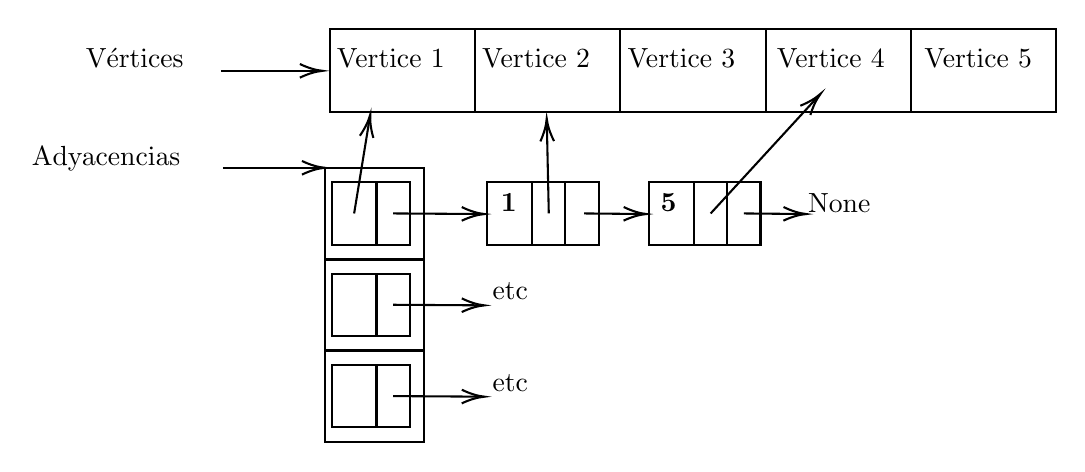
\begin{tikzpicture}[x=0.75pt,y=0.75pt,yscale=-1,xscale=1]
%uncomment if require: \path (0,300); %set diagram left start at 0, and has height of 300

%Shape: Rectangle [id:dp029559324877713067] 
\draw   (162,41) -- (232,41) -- (232,81) -- (162,81) -- cycle ;
%Shape: Rectangle [id:dp04407865842437819] 
\draw   (232,41) -- (302,41) -- (302,81) -- (232,81) -- cycle ;
%Shape: Rectangle [id:dp758311227719076] 
\draw   (302,41) -- (372,41) -- (372,81) -- (302,81) -- cycle ;
%Shape: Rectangle [id:dp02697734059652901] 
\draw   (372,41) -- (442,41) -- (442,81) -- (372,81) -- cycle ;
%Shape: Rectangle [id:dp1683889708060069] 
\draw   (442,41) -- (512,41) -- (512,81) -- (442,81) -- cycle ;
%Shape: Rectangle [id:dp019407999320991243] 
\draw   (238,115) -- (259.57,115) -- (259.57,145) -- (238,145) -- cycle ;
%Shape: Rectangle [id:dp6785514746075956] 
\draw   (259.57,115) -- (275.57,115) -- (275.57,145) -- (259.57,145) -- cycle ;
%Shape: Rectangle [id:dp36811881228026677] 
\draw   (275.57,115) -- (291.57,115) -- (291.57,145) -- (275.57,145) -- cycle ;
%Shape: Rectangle [id:dp6873241151839142] 
\draw   (163,115) -- (184.57,115) -- (184.57,145) -- (163,145) -- cycle ;
%Shape: Rectangle [id:dp12640905816779635] 
\draw   (184.57,115) -- (200.57,115) -- (200.57,145) -- (184.57,145) -- cycle ;
%Straight Lines [id:da47400455019003696] 
\draw    (192.57,130) -- (234.57,130.27) ;
\draw [shift={(236.57,130.29)}, rotate = 180.37] [color={rgb, 255:red, 0; green, 0; blue, 0 }  ][line width=0.75]    (10.93,-3.29) .. controls (6.95,-1.4) and (3.31,-0.3) .. (0,0) .. controls (3.31,0.3) and (6.95,1.4) .. (10.93,3.29)   ;
%Shape: Rectangle [id:dp4030712191532335] 
\draw   (316,115) -- (337.57,115) -- (337.57,145) -- (316,145) -- cycle ;
%Shape: Rectangle [id:dp4013828854449373] 
\draw   (337.57,115) -- (353.57,115) -- (353.57,145) -- (337.57,145) -- cycle ;
%Shape: Rectangle [id:dp6459203533406854] 
\draw   (353.57,115) -- (369.57,115) -- (369.57,145) -- (353.57,145) -- cycle ;
%Straight Lines [id:da669287611170156] 
\draw    (284.57,130) -- (312.57,130.27) ;
\draw [shift={(314.57,130.29)}, rotate = 180.55] [color={rgb, 255:red, 0; green, 0; blue, 0 }  ][line width=0.75]    (10.93,-3.29) .. controls (6.95,-1.4) and (3.31,-0.3) .. (0,0) .. controls (3.31,0.3) and (6.95,1.4) .. (10.93,3.29)   ;
%Shape: Rectangle [id:dp5523723109528451] 
\draw   (159.57,108) -- (207.57,108) -- (207.57,152.29) -- (159.57,152.29) -- cycle ;
%Shape: Rectangle [id:dp9213052722208128] 
\draw   (163,159) -- (184.57,159) -- (184.57,189) -- (163,189) -- cycle ;
%Shape: Rectangle [id:dp03361894910407903] 
\draw   (184.57,159) -- (200.57,159) -- (200.57,189) -- (184.57,189) -- cycle ;
%Straight Lines [id:da2744087751457245] 
\draw    (192.57,174) -- (234.57,174.27) ;
\draw [shift={(236.57,174.29)}, rotate = 180.37] [color={rgb, 255:red, 0; green, 0; blue, 0 }  ][line width=0.75]    (10.93,-3.29) .. controls (6.95,-1.4) and (3.31,-0.3) .. (0,0) .. controls (3.31,0.3) and (6.95,1.4) .. (10.93,3.29)   ;
%Shape: Rectangle [id:dp6669366229773146] 
\draw   (159.57,152) -- (207.57,152) -- (207.57,196.29) -- (159.57,196.29) -- cycle ;
%Straight Lines [id:da17475796169053592] 
\draw    (361.57,130) -- (389.57,130.27) ;
\draw [shift={(391.57,130.29)}, rotate = 180.55] [color={rgb, 255:red, 0; green, 0; blue, 0 }  ][line width=0.75]    (10.93,-3.29) .. controls (6.95,-1.4) and (3.31,-0.3) .. (0,0) .. controls (3.31,0.3) and (6.95,1.4) .. (10.93,3.29)   ;
%Straight Lines [id:da6312811023070157] 
\draw    (173.79,130) -- (181.25,84.26) ;
\draw [shift={(181.57,82.29)}, rotate = 99.27] [color={rgb, 255:red, 0; green, 0; blue, 0 }  ][line width=0.75]    (10.93,-3.29) .. controls (6.95,-1.4) and (3.31,-0.3) .. (0,0) .. controls (3.31,0.3) and (6.95,1.4) .. (10.93,3.29)   ;
%Straight Lines [id:da8106808504994962] 
\draw    (267.57,130) -- (266.62,86.29) ;
\draw [shift={(266.57,84.29)}, rotate = 88.75] [color={rgb, 255:red, 0; green, 0; blue, 0 }  ][line width=0.75]    (10.93,-3.29) .. controls (6.95,-1.4) and (3.31,-0.3) .. (0,0) .. controls (3.31,0.3) and (6.95,1.4) .. (10.93,3.29)   ;
%Straight Lines [id:da25565111637928095] 
\draw    (345.57,130) -- (397.22,73.76) ;
\draw [shift={(398.57,72.29)}, rotate = 132.56] [color={rgb, 255:red, 0; green, 0; blue, 0 }  ][line width=0.75]    (10.93,-3.29) .. controls (6.95,-1.4) and (3.31,-0.3) .. (0,0) .. controls (3.31,0.3) and (6.95,1.4) .. (10.93,3.29)   ;
%Shape: Rectangle [id:dp6269027651612935] 
\draw   (163,203) -- (184.57,203) -- (184.57,233) -- (163,233) -- cycle ;
%Shape: Rectangle [id:dp04605207955019619] 
\draw   (184.57,203) -- (200.57,203) -- (200.57,233) -- (184.57,233) -- cycle ;
%Straight Lines [id:da5483259148493369] 
\draw    (192.57,218) -- (234.57,218.27) ;
\draw [shift={(236.57,218.29)}, rotate = 180.37] [color={rgb, 255:red, 0; green, 0; blue, 0 }  ][line width=0.75]    (10.93,-3.29) .. controls (6.95,-1.4) and (3.31,-0.3) .. (0,0) .. controls (3.31,0.3) and (6.95,1.4) .. (10.93,3.29)   ;
%Shape: Rectangle [id:dp4696407316643838] 
\draw   (159.57,196) -- (207.57,196) -- (207.57,240.29) -- (159.57,240.29) -- cycle ;
%Straight Lines [id:da06390681702517043] 
\draw    (109.57,61.29) -- (156.57,61.29) ;
\draw [shift={(158.57,61.29)}, rotate = 180] [color={rgb, 255:red, 0; green, 0; blue, 0 }  ][line width=0.75]    (10.93,-3.29) .. controls (6.95,-1.4) and (3.31,-0.3) .. (0,0) .. controls (3.31,0.3) and (6.95,1.4) .. (10.93,3.29)   ;
%Straight Lines [id:da13188860148094306] 
\draw    (110.57,108) -- (157.57,108) ;
\draw [shift={(159.57,108)}, rotate = 180] [color={rgb, 255:red, 0; green, 0; blue, 0 }  ][line width=0.75]    (10.93,-3.29) .. controls (6.95,-1.4) and (3.31,-0.3) .. (0,0) .. controls (3.31,0.3) and (6.95,1.4) .. (10.93,3.29)   ;

% Text Node
\draw (43,49) node [anchor=north west][inner sep=0.75pt]   [align=left] {Vértices};
% Text Node
\draw (164,49) node [anchor=north west][inner sep=0.75pt]   [align=left] {Vertice 1};
% Text Node
\draw (234,49) node [anchor=north west][inner sep=0.75pt]   [align=left] {Vertice 2};
% Text Node
\draw (304,49) node [anchor=north west][inner sep=0.75pt]   [align=left] {Vertice 3};
% Text Node
\draw (376,49) node [anchor=north west][inner sep=0.75pt]   [align=left] {Vertice 4};
% Text Node
\draw (447,49) node [anchor=north west][inner sep=0.75pt]   [align=left] {Vertice 5};
% Text Node
\draw (17,96) node [anchor=north west][inner sep=0.75pt]   [align=left] {Adyacencias};
% Text Node
\draw (391,119) node [anchor=north west][inner sep=0.75pt]   [align=left] {None};
% Text Node
\draw (243,119) node [anchor=north west][inner sep=0.75pt]   [align=left] {\textbf{1}};
% Text Node
\draw (320,119) node [anchor=north west][inner sep=0.75pt]   [align=left] {\textbf{5}};
% Text Node
\draw (239,162) node [anchor=north west][inner sep=0.75pt]   [align=left] {etc};
% Text Node
\draw (239,206) node [anchor=north west][inner sep=0.75pt]   [align=left] {etc};


\end{tikzpicture}

Como alternativa a las listas se pueden usar diccionarios:

\begin{pyverbatim}[][frame=single]
vertices: Dict = {id1: valor_vertice_1,
                  id2: valor_vertice_2,
                  id3: valor_vertice_3,
                  ...
                  }
                
adyacencias: Dict = {id1: lista_adyacentes_del_vertice_id1, # Lista simplemente enlazada
                     id2: lista_adyacentes_del_vertice_id2,
                     id3: lista_adyacentes_del_vertice_id3,
                     ...
                     }
\end{pyverbatim}


\

Una modificación del algoritmo es el \textbf{algoritmo de Coste Uniforme} (sección \ref{subsec:problemasbusqueda}) que busca el camino de menor coste entre el nodo inicial y uno nodo destino. En este caso, en el paso 3.b) se comprobará si el nodo $u$ es un nodo destino. Si lo fuera, entonces finaliza el algoritmo. Es muy fácil obtener el algoritmo de Coste Uniforme usando el código del Ejercicio \ref{ejerc:laberintos}, que ya has implementado.

\

El \textbf{algoritmo A*} (sección \ref{subsec:problemasbusqueda}, ejercicio  \ref{ejer:Astar}),  puede usar este algoritmo para calcular el valor heurístico, $h(n)$, de cada nodo al nodo origen. Notar que para el A*, su punto destino es el origen de Dijkstra.

\


Un ejemplo de uso lo encontramos en problemas de transporte para encontrar el camino más corto entre un origen y un destino (p.e. cuando Google Maps te indica la cantidad de Kms que vas a recorre entre dos puntos geográficos). En videojuegos se usa para que los personajes no controlados por el jugador encuentren el camino más corto desde donde se encuentran hasta donde tú los mandes o para buscar el camino más corto para !`matarte!.

% - - - - - - - - - - - - - - - - - - - - - - - - - - - - - - - - - - - - - - - - - - - -

%\input ejercicios/05-Funciones/AleatoriosSol.tex





%%%%%%%%%%%%%%%%%%%%%%%%%%%%%%%%%%%%%%%%%%%%%%%%%% 
\separacion
\section{Árboles Generadores} 
\objetivo{2}{-}{Algoritmo de Prim}

Implementa el algoritmo de Prim que permite obtener el grafo generador de menor costo de un grafo.

\begin{enumerate}
\item Elegir un nodo origen.
\item Agregar el nodo a la lista de visitados.
\item Agregar sus adyacentes a la lista $L$, que es una lista ordenada de los nodos (por costes).
\item Mientras que la lista $L$ no esté vacía:
	\begin{enumerate}
	\item Extraer el mejor nodo de $L$
	\item Si el nodo no está en la lista de visitados
		\begin{enumerate}
		\item Agregar a la lista ordenada $L$ los adyacentes del nodo que no hayan sido visitados.
		\item Agregar el nodo al árbol solución.
		\end{enumerate}
	\end{enumerate}
\item Retornar el árbol solución.
\end{enumerate}


Un ejemplo de uso es el siguiente. Imagina que una empresa eléctrica tiene que hacer un nuevo tendido de cables que debe de pasar por varias localidades empezando desde una localidad que es la que recibe el suministro. En el modelo (grafo), toda localidad se conecta con otra localidad siempre que sea viable hacer un tendido entre las dos (lo que conllevará un coste positivo). El resultado final es un grafo no dirigido pesado. El algoritmo de Prim obtiene un árbol que contiene a todas las localidades, cada una se conectará con otra siempre que sea la conexión más económica de entre todas las posibles conexiones.

% - - - - - - - - - - - - - - - - - - - - - - - - - - - - - - - - - - - - - - - - - - - -

%\input ejercicios/05-Funciones/AleatoriosSol.tex










\separacion


